\documentclass[border=5pt]{standalone}
\usepackage{tikz}

\begin{document}

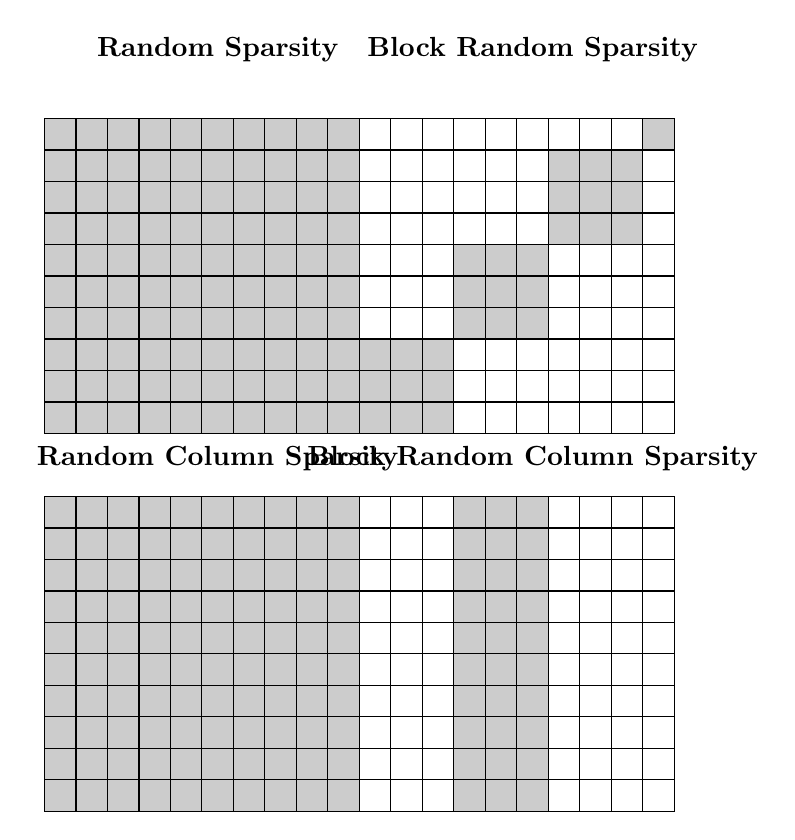
\begin{tikzpicture}[
    cell/.style={
        draw,
        minimum size=0.4cm,
        inner sep=0pt,
        outer sep=0pt
    },
    filled/.style={
        cell,
        fill=gray!40
    },
    empty/.style={
        cell,
        fill=white
    },
    title/.style={
        font=\bfseries,
        anchor=south
    }
]

% 定义随机数种子,确保每次编译结果一致
\pgfmathsetseed{12345}

% 常量定义
\def\gridsize{10} % 10x10网格
\def\blocksize{3} % 块大小
\def\sparsity{0.2} % 稀疏率(非零元素比例)

% Random Sparsity
\node[title] at (5*0.4, 11*0.4) {Random Sparsity};
\foreach \i in {0,...,\numexpr\gridsize-1\relax} {
    \foreach \j in {0,...,\numexpr\gridsize-1\relax} {
        \pgfmathrandom{0}{100}
        \pgfmathsetmacro{\randval}{int(\pgfmathresult)}
        \ifnum\randval<20
            \node[filled] at (\i*0.4, \j*0.4) {};
        \else
            \node[empty] at (\i*0.4, \j*0.4) {};
        \fi
    }
}

% Block Random Sparsity
\node[title] at (15*0.4, 11*0.4) {Block Random Sparsity};
\foreach \i in {0,...,\numexpr\gridsize-1\relax} {
    \foreach \j in {0,...,\numexpr\gridsize-1\relax} {
        \pgfmathrandom{0}{100}
        \pgfmathsetmacro{\randblock}{int(\pgfmathresult)}
        \pgfmathtruncatemacro{\blocki}{int(\i/\blocksize)}
        \pgfmathtruncatemacro{\blockj}{int(\j/\blocksize)}
        \pgfmathsetmacro{\inblock}{mod(\blocki*3+\blockj, 4) == 0 ? 1 : 0}
        \ifnum\randblock<30
            \ifnum\inblock=1
                \node[filled] at ({(\i+10)*0.4}, \j*0.4) {};
            \else
                \node[empty] at ({(\i+10)*0.4}, \j*0.4) {};
            \fi
        \else
            \node[empty] at ({(\i+10)*0.4}, \j*0.4) {};
        \fi
    }
}

% Random Column Sparsity
\node[title] at (5*0.4, 0*0.4-0.8) {Random Column Sparsity};
\foreach \i in {0,...,\numexpr\gridsize-1\relax} {
    \pgfmathrandom{0}{100}
    \pgfmathsetmacro{\randcol}{int(\pgfmathresult)}
    \ifnum\randcol<30
        \foreach \j in {0,...,\numexpr\gridsize-1\relax} {
            \node[filled] at (\i*0.4, {(\j-12)*0.4}) {};
        }
    \else
        \foreach \j in {0,...,\numexpr\gridsize-1\relax} {
            \node[empty] at (\i*0.4, {(\j-12)*0.4}) {};
        }
    \fi
}

% Block Random Column Sparsity
\node[title] at (15*0.4, 0*0.4-0.8) {Block Random Column Sparsity};
\foreach \i in {0,...,\numexpr\gridsize-1\relax} {
    \pgfmathtruncatemacro{\blocki}{int(\i/\blocksize)}
    \pgfmathrandom{0}{100}
    \pgfmathsetmacro{\randcol}{int(\pgfmathresult)}
    \ifnum\randcol<40
        \ifnum\blocki=1
            \foreach \j in {0,...,\numexpr\gridsize-1\relax} {
                \node[filled] at ({(\i+10)*0.4}, {(\j-12)*0.4}) {};
            }
        \else
            \foreach \j in {0,...,\numexpr\gridsize-1\relax} {
                \node[empty] at ({(\i+10)*0.4}, {(\j-12)*0.4}) {};
            }
        \fi
    \else
        \foreach \j in {0,...,\numexpr\gridsize-1\relax} {
            \node[empty] at ({(\i+10)*0.4}, {(\j-12)*0.4}) {};
        }
    \fi
}

\end{tikzpicture}

\end{document}